\documentclass[aspectratio=169]{../latex_main/tntbeamer}  % you can pass all options of the beamer class, e.g., 'handout' or 'aspectratio=43'
\usepackage{dsfont}
\usepackage{bm}
\usepackage[english]{babel}
\usepackage[T1]{fontenc}
%\usepackage[utf8]{inputenc}
\usepackage{graphicx}
\graphicspath{ {./figures/} }
\usepackage{algorithm}
\usepackage[ruled,vlined,algo2e,linesnumbered]{algorithm2e}
\usepackage{hyperref}
\usepackage{booktabs}
\usepackage{mathtools}

\usepackage{amsmath,amssymb}

\DeclareMathOperator*{\argmax}{arg\,max}
\DeclareMathOperator*{\argmin}{arg\,min}

\usepackage{pgfplots}
\pgfplotsset{compat=1.16}
\usepackage{tikz}
\usetikzlibrary{trees} 
\usetikzlibrary{shapes.geometric}
\usetikzlibrary{positioning,shapes,shadows,arrows,calc,mindmap}
\usetikzlibrary{positioning,fadings,through}
\usetikzlibrary{decorations.pathreplacing}
\usetikzlibrary{intersections}
\pgfdeclarelayer{background}
\pgfdeclarelayer{foreground}
\pgfsetlayers{background,main,foreground}
\tikzstyle{activity}=[rectangle, draw=black, rounded corners, text centered, text width=8em]
\tikzstyle{data}=[rectangle, draw=black, text centered, text width=8em]
\tikzstyle{myarrow}=[->, thick, draw=black]

% Define the layers to draw the diagram
\pgfdeclarelayer{background}
\pgfdeclarelayer{foreground}
\pgfsetlayers{background,main,foreground}

% Requires XeLaTeX or LuaLaTeX
\usepackage{unicode-math}

\usepackage{fontspec}
%\setsansfont{Arial}
\setsansfont{RotisSansSerifStd}[ 
Path=../latex_main/fonts/,
Extension = .otf,
UprightFont = *-Regular,  % or *-Light
BoldFont = *-ExtraBold,  % or *-Bold
ItalicFont = *-Italic
]
\setmonofont{Cascadia Mono}[
Scale=0.8
]

% scale factor adapted; mathrm font added (Benjamin Spitschan @TNT, 2021-06-01)
%\setmathfont[Scale=1.05]{Libertinus Math}
%\setmathrm[Scale=1.05]{Libertinus Math}

% other available math fonts are (not exhaustive)
% Latin Modern Math
% XITS Math
% Libertinus Math
% Asana Math
% Fira Math
% TeX Gyre Pagella Math
% TeX Gyre Bonum Math
% TeX Gyre Schola Math
% TeX Gyre Termes Math

% Literature References
\newcommand{\lit}[2]{\href{#2}{\footnotesize\color{black!60}[#1]}}

%%% Beamer Customization
%----------------------------------------------------------------------
% (Don't) Show sections in frame header. Options: 'sections', 'sections light', empty
\setbeamertemplate{headline}{empty}

% Add header logo for normal frames
\setheaderimage{
	% 
\includegraphics[height=\logoheight]{figures/TNT_darkv4.pdf}
	
\includegraphics[height=\logoheight]{../latex_main/figures/luh_logo_rgb_0_80_155.pdf}
	% 
\includegraphics[height=\logoheight]{figures/logo_tntluh.pdf}
}

% Header logo for title page
\settitleheaderimage{
	% 
\includegraphics[height=\logoheight]{figures/TNT_darkv4.pdf}
	
\includegraphics[height=\logoheight]{../latex_main/figures/luh_logo_rgb_0_80_155.pdf}
	% 
\includegraphics[height=\logoheight]{figures/logo_tntluh.pdf}
}

% Title page: tntdefault 
\setbeamertemplate{title page}[tntdefault]  % or luhstyle
% Add optional title image here
%\addtitlepageimagedefault{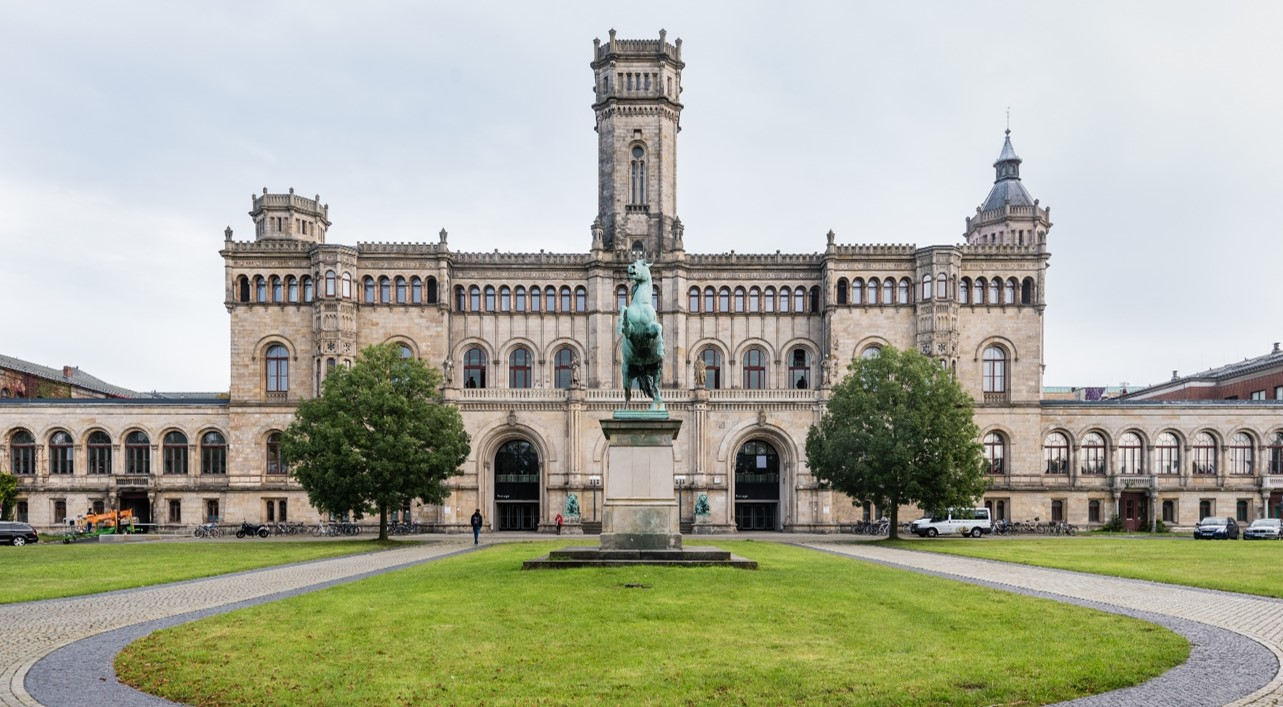
\includegraphics[width=0.65\textwidth]{figures/luh_default_presentation_title_image.jpg}}

% Title page: luhstyle
% \setbeamertemplate{title page}[luhstyle]
% % Add optional title image here
% \addtitlepageimage{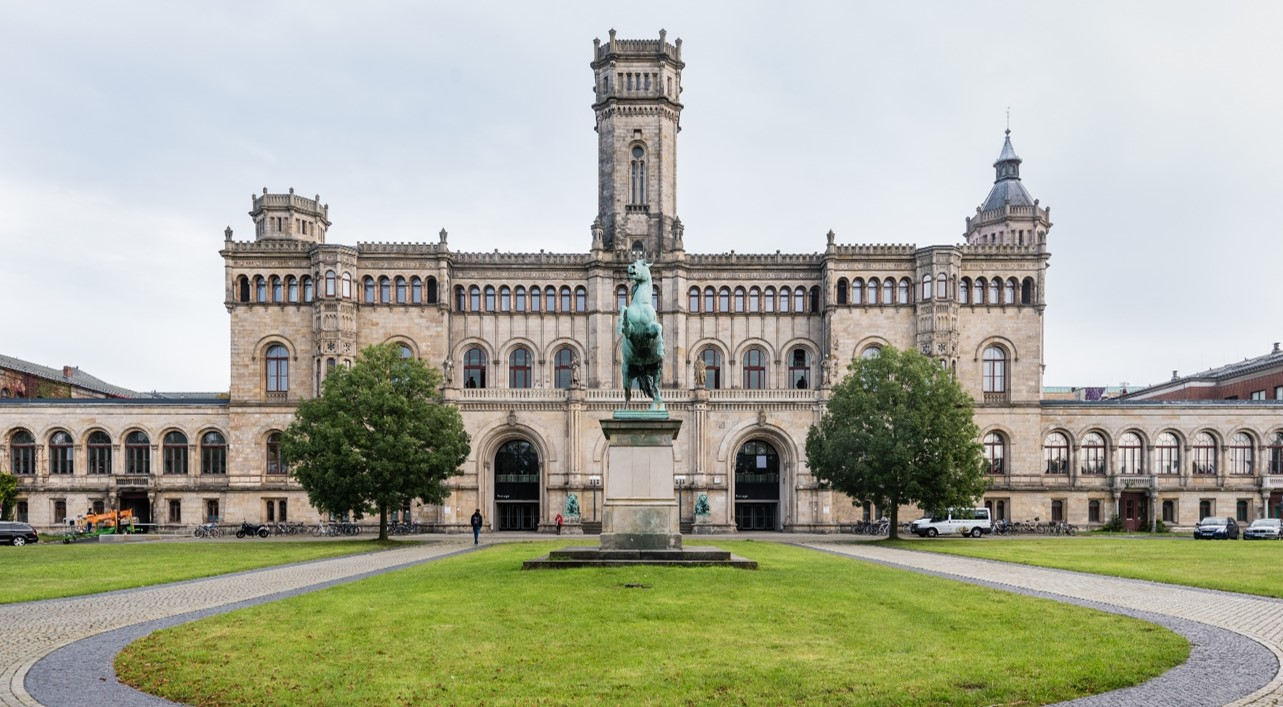
\includegraphics[width=0.75\textwidth]{figures/luh_default_presentation_title_image.jpg}}

\author[Lindauer \& Anand]{Marius Lindauer and Avishek Anand\\[1em]
	
\includegraphics[height=\logoheight]{../latex_main/figures/luh_logo_rgb_0_80_155.pdf}\qquad

\includegraphics[height=\logoheight]{../latex_main/figures/TNT_darkv4}\qquad

\includegraphics[height=\logoheight]{../latex_main/figures/L3S.jpg}	}
\date{Winter Term 2021
}


%%% Custom Packages
%----------------------------------------------------------------------
% Create dummy content
\usepackage{blindtext}

% Adds a frame with the current page layout. Just call \layout inside of a frame.
\usepackage{layout}


\title[Introduction]{iML: Local Explanations}
\subtitle{Anchors}

%\institute{}


\begin{document}
	
	\maketitle

	%-----------------------------------------------------------------------------------------------------------------------------


\begin{frame}{Anchors \lit{Ribeiro et al. 2018}{https://homes.cs.washington.edu/~marcotcr/aaai18.pdf}}
\begin{itemize}
		\item local explanation of a single prediction $x$
		\begin{itemize}
		    \item successor of LIME
		\end{itemize}
		\pause
		\item[$\leadsto$] finding a rule that "anchors" the prediction
		\item[$\leadsto$] "anchors" i.e., focus on the feature value responsible for the prediction
		\pause
		\smallskip
		\item (again) perturbation-based strategy for generation of local explanations
		\pause
		\smallskip
		\item explanations are expressed as IF-THEN rules, a.k.a. anchors
\end{itemize}
\end{frame}

%---------------------------------------------------------

\begin{frame}[fragile]{Example Anchor}
\begin{itemize}
        \item Example from Titanic dataset: Who would survive?
		\item Input $x$ = \{'age': 20, 'sex': female, 'class': first, 'ticketPrice': 300, \ldots\}
		\item Prediction: 'survived': True
		\item Exemplary anchor:
\end{itemize}

\begin{verbatim}
    IF SEX = female
    AND Class = first
    THEN PREDICT Survived = true
    WITH PRECISION 97%
    AND COVERAGE 15%
\end{verbatim}

\end{frame}

%---------------------------------------------------------

\begin{frame}[c]{Discussion of Anchors}

\begin{itemize}
    \item very easy to understand
    \smallskip
    \pause
    \item includes the notion of coverage
    \begin{itemize}
        \item[$\leadsto$] too how much of the (feasible) space would the rule apply to
        \item faithful by design
        \item should be maximized!
    \end{itemize}
    \smallskip
    \pause
    \item includes precision:
    \begin{itemize}
        \item[$\leadsto$] precision of the rule in its subspace
        \item should be maximized!
    \end{itemize}
    \smallskip
    \pause
    \item Trade-off between high coverage and high precision
    \begin{itemize}
        \item maximal coverage would be a constant predictor for the entire space $\leadsto$ poor precision
        \item maximal precision would lead to a very small subspace $\leadsto$ small coverage
    \end{itemize}
    
\end{itemize}


\end{frame}

%---------------------------------------------------------

\begin{frame}[c]{Visualisation of an Anchor}

\centering
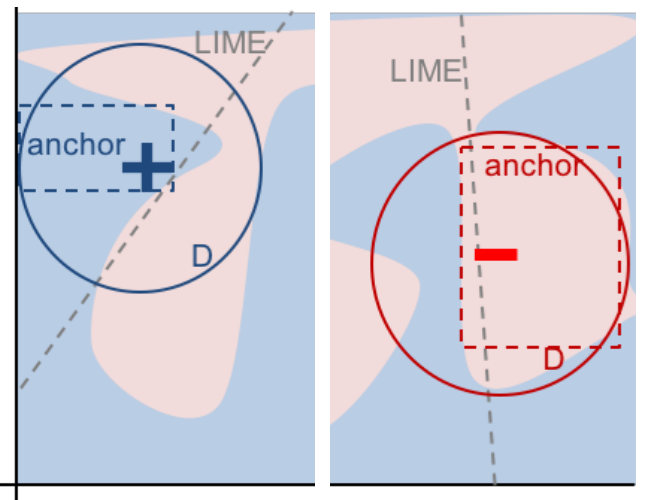
\includegraphics[width=0.5\textwidth]{./figure/anchors-visualization_orig.png}\\
Source: \lit{Ribeiro et al. 2018}{https://homes.cs.washington.edu/~marcotcr/aaai18.pdf}

\end{frame}

%---------------------------------------------------------

\begin{frame}[c]{Definition Anchor}

An anchor is defined as:

\begin{equation}
    \mathbb{E}_{\mathcal{D}_x(z\mid A)} [\mathbb{1}_{f(x) = f(z)}] \leq \tau, \text{ s.t. } A(x) = 1
\end{equation}

with 

\begin{itemize}
    \item x being the instance at hand (to be explained)
    \item A being a set of predicates, i.e.,  the anchor's if statement
    \begin{itemize}
        \item side constraint: $A(x)$ has to be satisfied for the given feature vector $x$
    \end{itemize}
    \item $f$ being the predictive model to be explained -- can be queried
    \item $\mathcal{D}(\cdot \mid A)$ indicates the distribution of neighbors of $x$, matching A.
    \item $0 \leq \tau \leq 1$ specifies a precision threshold
\end{itemize}

\end{frame}

%---------------------------------------------------------

\begin{frame}[c]{Relaxing Anchor's Definition}

\begin{itemize}
    \item combinatorial problem to find an anchor
    \item hard to evaluate precision in a continuous or large feature space
    \item Relaxation of the problem:
\end{itemize}

$$P( prec(A) \geq \tau) \geq 1  - \delta \text{ with } prec(A)  = \mathbb{E}_{\mathcal{D}_x(z\mid A)} [\mathbb{1}_{f(x) = f(z)}] $$

with $\delta$ being a probability threshold to each desired precision.

\pause
\medskip

$\leadsto$ If $\delta$ is very small:
\begin{description}
    \item[a)] very hard to find $A$
    \item[b)] high confidence to that precision is achieved
\end{description}
(similar to $\alpha$ in a statistical hypothesis test.)

\end{frame}

%---------------------------------------------------------

\begin{frame}[c]{Considering Coverage}

\begin{itemize}
    \item Additionaly, we want to maximize the coverage of the anchor\\ w.r.t. to the neighborhood distribution $\mathcal{D}$
\end{itemize}

$$\max_{A} cov(A) = \max_{A} \mathbb{E}_{\mathcal{D}(z)[A(z)]} $$


\end{frame}

%---------------------------------------------------------

\begin{frame}[c]{Final Anchor Optimization Problem}

\begin{equation}
\max_{A} cov(A) \text{ s.t. } P(prec(A) \geq \tau) \geq 1 - \delta
\end{equation}

\begin{itemize}
    \item Bound $\tau$ on precision with confidence $\delta$
    \item and maximization of coverage
\end{itemize}


\end{frame}

%---------------------------------------------------------

\begin{frame}[c]{Anchor Algorithm Outline \lit{Ribeiro et al. 2018}{https://homes.cs.washington.edu/~marcotcr/aaai18.pdf}}

\begin{enumerate}

    \item \textbf{Initialization} One anchor for each $x_i$ in given $x$
    \item \textbf{Candidate Update} Add another $x_i$ not considered in A so far
    \item \textbf{Best Candidate Identification} use multi-armed-bandit approach to focus investment in model predictions into promising anchors 
    \item \textbf{Selection} Use beam search to only consider $B$ best anchors in each iteration 
\end{enumerate}

\end{frame}


\end{document}